%%%%%%%%%%%%%%%%%%%%%%%%%%%%%%%%%%%%%%%%%%%%%%%%%%%%%%%%%%%%%%%
%
% Welcome to Overleaf --- just edit your LaTeX on the left,
% and we'll compile it for you on the right. If you open the
% 'Share' menu, you can invite other users to edit at the same
% time. See www.overleaf.com/learn for more info. Enjoy!
%
%%%%%%%%%%%%%%%%%%%%%%%%%%%%%%%%%%%%%%%%%%%%%%%%%%%%%%%%%%%%%%%
% -------------------------------------------------------------------------------
% This is all preamble stuff that you don't have to worry about.
% Head down to where it says "Enter your name here"
% -------------------------------------------------------------------------------
 
\documentclass[12pt]{article}
 
\usepackage[margin=1in]{geometry} 
\usepackage{amsmath,amsthm,amssymb}
\usepackage{graphicx}
\usepackage{enumerate}
\usepackage[names]{xcolor}
\usepackage[multiple,hang,flushmargin]{footmisc}
\usepackage{lastpage}
\usepackage{tikz}
\usepackage{listings}
\usepackage[parfill]{parskip}
\parskip=\baselineskip

 
\newenvironment{question}[2][Question]{\begin{trivlist}
\item[\hskip \labelsep {\bfseries #1}\hskip \labelsep {\bfseries #2.}]}{\end{trivlist}}
\newenvironment{solution}[1][Solution:]{\begin{trivlist}
\item[\hskip \labelsep {\bfseries #1}\hskip \labelsep {\bfseries}]\color{blue}}{\end{trivlist}}

\usepackage{fancyhdr}
\pagestyle{fancy}
\rhead{Due: \duedate}
\lhead{CSC250 - Midterm}
\cfoot{p. \thepage \ of \pageref{LastPage}}
\renewcommand{\headrulewidth}{0.4pt}
\renewcommand{\footrulewidth}{0.4pt}

 
\begin{document}
\newcommand{\duedate}{11:59PM EST Thursday March 27, 2025}

% --------------------------------------------------------------------------------------------
%  Great, now skip ahead to where you see *** START EXAM HERE ***
% --------------------------------------------------------------------------------------------

\topskip0pt
\vspace*{\fill}
\begin{center}
\fbox{\fbox{\parbox{5.5in}{\begin{center}
\vspace{1em}
This is the first of two examinations for\\ \textbf{CSC250: Theory of Computation}\\ as taught by Pablo Frank Bolton in Spring 2025.\\
\vspace{1em}
\begin{itemize}
  \item your own notes
  \item lecture slides / videos
  \item scribe notes
  \item homework solutions
  \item any of the recommended textbooks
\end{itemize}
\vspace{1em}
\textbf{Honor code: no other resources are permitted during this exam.}\\
This includes (but is not limited to): online materials, tutors, teaching assistants, and other students.
\end{center}
\vspace{5em}
 \ \ \ YOUR NAME: \underline{\hspace{10cm}}
\vspace{3em}}}}
\end{center}
\vspace{3em}
\vspace*{\fill}


% ---------------------------------------
%   *** START EXAM HERE ***
% ---------------------------------------

\clearpage
\bigskip

\textbf{How to answer this exam}

\begin{itemize}
    \item There are a \textbf{total of 50 points}. There is a bonus question at the end (about Linear Temporal Logic worth 2 additional points)
    \item Read the questions twice. Sometimes, you answer something other than what is asked, so make sure you understand what it is I am asking for.
    \item Consider the following 4 principles for answering:
    \begin{itemize}
        \item \textbf{Correctness}: first and foremost, answer with truthful statements only.
        \item \textbf{Completeness}: check your answer to make sure you answered the whole question.
        \item \textbf{Clarity}: before answering, think about the structure of your response so that it is straightforward, simple, and it satisfies the two previous principles.
        \item \textbf{Conciseness}: longer is not better... it is in fact worse, so only answer what is asked for, in a simple way, and as long as it is correct and complete, it will be good enough.
    \end{itemize}

\textbf{IMPORTANT}: If I cannot read or see your answers (images too small or wording is confusing, I will take points away).
\end{itemize}


\bigskip

\begin{question}{0}\textbf{Getting in the Groove} (0 points)
\begin{center}
\textit{Note: This question is optional, but strongly recommended.}
\end{center}
Educational research studies\footnote{\scriptsize{Lang, Jonas WB, and Jessica Lang. ``Priming competence diminishes the link between cognitive test anxiety and test performance: Implications for the interpretation of test scores.'' \textit{Psychological Science} 21.6 (2010): 811-819.}}\footnote{\scriptsize{Barrows, Jennifer, Samantha Dunn, and Carrie A. Lloyd. ``Anxiety, self-efficacy, and college exam grades.'' \textit{Universal Journal of Educational Research} 1.3 (2013): 204-208.}} have suggested that people perform better on tests when they spend a few minutes thinking about things they're good at before they begin.\\\\
In the space below, briefly tell us about a time when you were \textbf{really successful} at doing something challenging (it doesn't have to be related to this course). If you prefer, you can draw a picture instead of writing.\\
\vfill
\hfill
% 
\includegraphics[width=2in]{youcandoit.png}
\end{question}


% --------------------------------
% Big Picture
% --------------------------------
\clearpage
\begin{question}{1}\textbf{Big Picture  (6 points)}\\\\

Answer each of the following with no more than three sentences. Think before answering, and then provide a concise answer.


\begin{enumerate}[(a)]  
  \item \textit{(2 points) Why do we study Theory of Computation by checking membership of words into languages?}

    \begin{solution}
  Your solution here
    \end{solution}
    
 
  \item \textit{(2 points) In the Language categories map (the diagram with concentric ovals, each with a different language group), what differentiates the languages?}
 
    \begin{solution}
       Your solution here
    \end{solution}


        \item \textit{(2 points) As we progress from Regular Expressions, to CFGs to TMs, what makes each successive machine more powerful than the next?}
 
    \begin{solution}
       Your solution here
    \end{solution}
    
\end{enumerate}

\end{question}






% --------------------------------
% Logic
% --------------------------------
\clearpage
\begin{question}{2}\textbf{Propositional logic (4 points)}\\\\

Consider the following propositions:
\begin{eqnarray*}
  p & = & \texttt{It was raining.}\\
  q & = & \texttt{We played board games inside.}\\
  r & = & \texttt{We went to the beach.}
\end{eqnarray*}
Translate each of the following propositions into an English sentence.
\begin{enumerate}[(a)]  
  \item $q \vee r$\vspace{8em}
  \item $p \rightarrow q$\vspace{8em}
  \item $q \rightarrow \neg r$\vspace{8em}
  \item $p \wedge \neg r \rightarrow q$
\end{enumerate}
\end{question}


% \clearpage
% \begin{question}{1}\textbf{Valid or Invalid Reasoning} (6 points)\\\\
% For each of the following English arguments, express the argument in terms of
% propositional logic and briefly justify whether the argument is valid or invalid. Be sure to clearly label your propositions.
% \begin{enumerate}[(a)]  
%   \item \textit{When the weather is nice, Max either rides their bike on the rail trail or goes for a walk through the gardens (but never both on the same day). The weather is nice, and Max is going for a walk through the gardens. Therefore, Max will not ride their bike on the rail trail today.}

%     \begin{solution}
%   Your solution here
%     \end{solution}
    
 
%   \item \textit{When a student needs a book and a coffee,  they go to Neilson Library. There is a student at Neilson Library today. This means that they wanted to check out a book.}
 
%     \begin{solution}
%        Your solution here
%     \end{solution}
    
% \end{enumerate}
% \end{question}

% ---------------------------
% Regular expressions
% ---------------------------
\clearpage
\begin{question}{3}\textbf{Interpreting regular expressions (2 points)} \\\\

Describe the language matched by the following regular expression:
\[ (00 + 11 )^*\]
Note: Try to describe the resulting language, not the regular expression.
\end{question}

\begin{solution}
Your solution here
\end{solution}


\clearpage
\begin{question}{4}\textbf{Writing regular expressions (2 points)}\\\\
Consider the following language on the alphabet $\Sigma = \{0,1\}$:
\[L = \{w \ | \ w \texttt{ has even length and must contain the substring 0110}\}\]
Write a regular expression for $L$.
\end{question}

\begin{solution}
Your solution here
\end{solution}

% ----------------------
% Finite automata
% ----------------------
\clearpage
\begin{question}{5}\textbf{Interpreting  Finite Automata (6 points)}\\\\
Consider the following finite automaton:
% \begin{center}
%   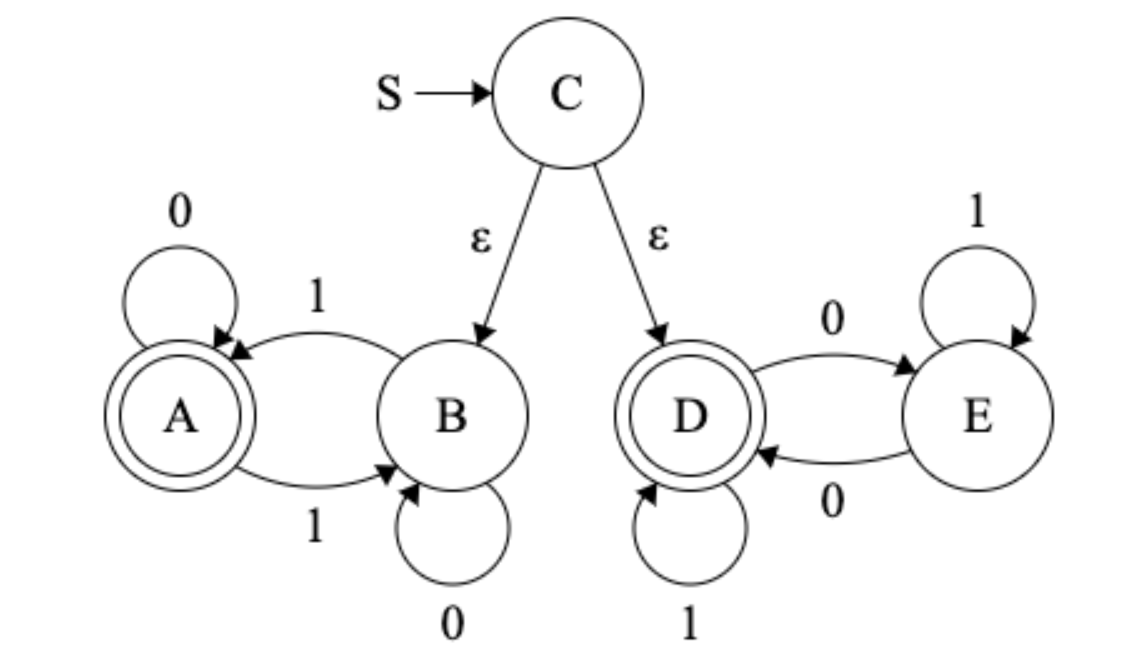
\includegraphics[width=0.6\textwidth]{q4-FA.png}
% \end{center}

\begin{center}
\begin{tikzpicture}[scale=0.2]
\tikzstyle{every node}+=[inner sep=0pt]
\draw [black] (31.7,-7) circle (3);
\draw (31.7,-7) node {$C$};
\draw [black] (14.1,-23.9) circle (3);
\draw (14.1,-23.9) node {$A$};
\draw [black] (14.1,-23.9) circle (2.4);
\draw [black] (25.1,-23.9) circle (3);
\draw (25.1,-23.9) node {$B$};
\draw [black] (38,-23.2) circle (3);
\draw (38,-23.2) node {$C$};
\draw [black] (38,-23.2) circle (2.4);
\draw [black] (50.3,-23.2) circle (3);
\draw (50.3,-23.2) node {$D$};
\draw [black] (25.9,-7) -- (28.7,-7);
\draw (25.4,-7) node [left] {$S$};
\fill [black] (28.7,-7) -- (27.9,-6.5) -- (27.9,-7.5);
\draw [black] (30.61,-9.79) -- (26.19,-21.11);
\fill [black] (26.19,-21.11) -- (26.95,-20.54) -- (26.02,-20.18);
\draw (27.65,-14.59) node [left] {$\epsilon$};
\draw [black] (32.79,-9.8) -- (36.91,-20.4);
\fill [black] (36.91,-20.4) -- (37.09,-19.48) -- (36.16,-19.84);
\draw (35.6,-14.24) node [right] {$\epsilon$};
\draw [black] (16.03,-21.642) arc (125.49136:54.50864:6.149);
\fill [black] (16.03,-21.64) -- (16.97,-21.59) -- (16.39,-20.77);
\draw (19.6,-20) node [above] {$0$};
\draw [black] (11.916,-21.86) arc (254.67738:-33.32262:2.25);
\draw (10.78,-17.06) node [above] {$1$};
\fill [black] (14.39,-20.93) -- (15.08,-20.29) -- (14.12,-20.02);
\draw [black] (22.92,-25.924) arc (-60.04879:-119.95121:6.65);
\fill [black] (22.92,-25.92) -- (21.98,-25.89) -- (22.48,-26.76);
\draw (19.6,-27.31) node [below] {$0$};
\draw [black] (26.722,-26.41) arc (60.6113:-227.3887:2.25);
\draw (26.12,-31.19) node [below] {$1$};
\fill [black] (24.09,-26.71) -- (23.27,-27.17) -- (24.14,-27.66);
\draw [black] (39.323,-25.88) arc (54:-234:2.25);
\draw (38,-30.45) node [below] {$0$};
\fill [black] (36.68,-25.88) -- (35.8,-26.23) -- (36.61,-26.82);
\draw [black] (40.197,-21.185) arc (121.25097:58.74903:7.621);
\fill [black] (48.1,-21.19) -- (47.68,-20.34) -- (47.16,-21.2);
\draw (44.15,-19.58) node [above] {$1$};
\draw [black] (47.841,-24.893) arc (-65.21379:-114.78621:8.804);
\fill [black] (40.46,-24.89) -- (40.98,-25.68) -- (41.39,-24.77);
\draw (44.15,-26.2) node [below] {$1$};
\draw [black] (49.796,-20.254) arc (217.43687:-70.56313:2.25);
\draw (53.06,-16.18) node [above] {$0$};
\fill [black] (52.33,-21.01) -- (53.27,-20.92) -- (52.66,-20.13);
\end{tikzpicture}
\end{center}

\begin{enumerate}[(a)]
    \item (1 point) What is the start state?
        \begin{solution}
            Your solution here
        \end{solution}
  \item (1 point) What is the set of accepting states?
        \begin{solution}
           Your solution here
        \end{solution}
  \item (2 points) What is a concise Regular Expression for this FA.
        \begin{solution}
            Your solution here
        \end{solution} 
  \item (2 points) Given your Regular Expression, what is a concise way to describe this language in English?
        \begin{solution}
            Your solution here
        \end{solution}  
  
\end{enumerate}
\end{question}

\clearpage
\begin{question}{6}\textbf{Building Finite Automata (6 points)}\\\\

Draw the transition diagram for a finite automaton that recognizes each of the following languages. In all cases, the alphabet is $\Sigma = \{0,1\}$.
\begin{enumerate}[(a)]
  \item $\{ w \in \Sigma^* \ | \ w \texttt{ begins with } 0 \texttt{ and ends with } 1 \}$.
\begin{solution}
\;
Your solution here
\end{solution} 

  \item $\{ w \in \Sigma^* \ | \ w \texttt{ contains an odd number of } 0s \}$.
\begin{solution}
\;
Your solution here
\end{solution}  
  
  \item $\{ w \in \Sigma^* \ | \ w \texttt{ does not contain the substring } 11 \}$.
\begin{solution}
\;
Your solution here
\end{solution}  

\end{enumerate}
\end{question}


\clearpage
\begin{question}{7}\textbf{Short proofs (8 points)}\\\\

Determine whether each of the following statements is \texttt{true} or \texttt{false}.\\ If it is \texttt{true}, provide a short proof. If it is \texttt{false}, give a counterexample.
\begin{enumerate}[(a)]
\item The intersection of two regular languages is finite.
\begin{solution}
    Your solution here
\end{solution}

\item The complement of a finite language must be regular.
\begin{solution}
    Your solution here
\end{solution}

\item No finite automaton can accept the empty string $\varepsilon$.
\begin{solution}
   Your solution here
\end{solution}

\item There exists some finite automaton that accepts the empty string $\varepsilon$.
\begin{solution}
    Your solution here   
\end{solution}
\end{enumerate}
\end{question}

\clearpage
\begin{question}{8}\textbf{Non-Regular Languages (6 points)}\\\\

Prove that the language: \[L_{ijk} = \{w \ | \ w = 0^i1^j0^k \; ; \quad i+j = k \; ; \quad i,j,k \geq 0 \} \] is \textbf{NOT} a regular language.

Note, example words in this language include $\epsilon, 00, 10, 0100, 0000, 1100, 001000$
\end{question}

\begin{solution}
Your solution here  
\end{solution}

\clearpage
\begin{question}{9}\textbf{Context-Free Languages(6 points)} \\\\

Prove that the language: \[L_{ijk} = \{w \ | \ w = 0^i1^j0^k \; ; \quad i+j = k \; ; \quad i,j,k \geq 0 \} \] is context-free.

Note, example words in this language include $\epsilon, 00, 10, 0100, 0000, 1100, 001000$
\end{question}


  \begin{solution}
 \;
 
 Your solution here
  \end{solution}

\clearpage
\begin{question}{10}\textbf{Decidable Languages (4 points)} \\\\
Prove that the language: \[L_{ijk} = \{w \ | \ w = 0^i1^j0^k \; ; \quad i+j = k \; ; \quad i,j,k \geq 0 \} \] is decidable.

Note, example words in this language include $\epsilon, 00, 10, 0100, 0000, 1100, 001000$
\end{question}

\begin{solution}
\;
Your solution here    
\end{solution}


\clearpage
\begin{question}{BONUS}\textbf{Linear Temporal Logic (2 points)} \\\\

\begin{itemize}
    \item (1 point) What does the following statement mean: \\
    $G(jump \; \rightarrow \; F ( \;deploy\; AND\; X( \;brace\; )\;   )\; )$

\begin{solution}
\;
Your solution here    
\end{solution}

\bigskip
    
    \item (1 point) Is the following sequence satisfying that statement?\\

\begin{table}[h!]
\begin{tabular}{|l|l|l|l|l|l|l|l|}
\hline
Time   & 1     & 2     & 3     & 4     & 5     & 6     & 7     \\ \hline
jump   & False & True  & False & True  & False & False & False \\ \hline
deploy & True  & False & False & False & True  & True  & False \\ \hline
brace  & False & False & False & True  & True  & False & False \\ \hline
\end{tabular}
\end{table}    

\begin{solution}
\;
Your solution here    
\end{solution}
    
\end{itemize}

\end{question}



\clearpage
\begin{center}
\vspace{-3em}
\textit{This page intentionally left blank as scratch paper.}
\end{center}


% --------------------------------------------------------------
%     You don't have to mess with anything below this line.
% --------------------------------------------------------------
 
\end{document}